\documentclass[11pt,a4paper]{report}
\usepackage[textwidth=37em,vmargin=30mm]{geometry}
\usepackage{calc,xunicode,amsmath,amssymb,paralist,enumitem,tabu,booktabs,datetime2,xeCJK,xeCJKfntef,listings}
\usepackage{tocloft,fancyhdr,tcolorbox,xcolor,graphicx,eso-pic,xltxtra,xelatexemoji}

\newcommand{\envyear}[0]{2025}
\newcommand{\envdatestr}[0]{2025-03-19}
\newcommand{\envfinaldir}[0]{webdb/2025/20250319/final}

\usepackage[hidelinks]{hyperref}
\hypersetup{
    colorlinks=false,
    pdfpagemode=FullScreen,
    pdftitle={Web Digest - \envdatestr}
}

\setlength{\cftbeforechapskip}{10pt}
\renewcommand{\cftchapfont}{\rmfamily\bfseries\large\raggedright}
\setlength{\cftbeforesecskip}{2pt}
\renewcommand{\cftsecfont}{\sffamily\small\raggedright}

\setdefaultleftmargin{2em}{2em}{1em}{1em}{1em}{1em}

\usepackage{xeCJK,xeCJKfntef}
\xeCJKsetup{PunctStyle=plain,RubberPunctSkip=false,CJKglue=\strut\hskip 0pt plus 0.1em minus 0.05em,CJKecglue=\strut\hskip 0.22em plus 0.2em}
\XeTeXlinebreaklocale "zh"
\XeTeXlinebreakskip = 0pt


\setmainfont{Brygada 1918}
\setromanfont{Brygada 1918}
\setsansfont{IBM Plex Sans}
\setmonofont{JetBrains Mono NL}
\setCJKmainfont{Noto Serif CJK SC}
\setCJKromanfont{Noto Serif CJK SC}
\setCJKsansfont{Noto Sans CJK SC}
\setCJKmonofont{Noto Sans CJK SC}

\setlength{\parindent}{0pt}
\setlength{\parskip}{8pt}
\linespread{1.15}

\lstset{
	basicstyle=\ttfamily\footnotesize,
	numbersep=5pt,
	backgroundcolor=\color{black!5},
	showspaces=false,
	showstringspaces=false,
	showtabs=false,
	tabsize=2,
	captionpos=b,
	breaklines=true,
	breakatwhitespace=true,
	breakautoindent=true,
	linewidth=\textwidth
}






\newcommand{\coverpic}[2]{
    % argv: itemurl, authorname
    Cover photo by #2~~(\href{#1}{#1})
}
\newcommand{\makeheader}[0]{
    \begin{titlepage}
        % \newgeometry{hmargin=15mm,tmargin=21mm,bmargin=12mm}
        \begin{center}
            
            \rmfamily\scshape
            \fontspec{BaskervilleF}
            \fontspec{Old Standard}
            \fontsize{59pt}{70pt}\selectfont
            WEB\hfill DIGEST
            
            \vfill
            % \vskip 30pt
            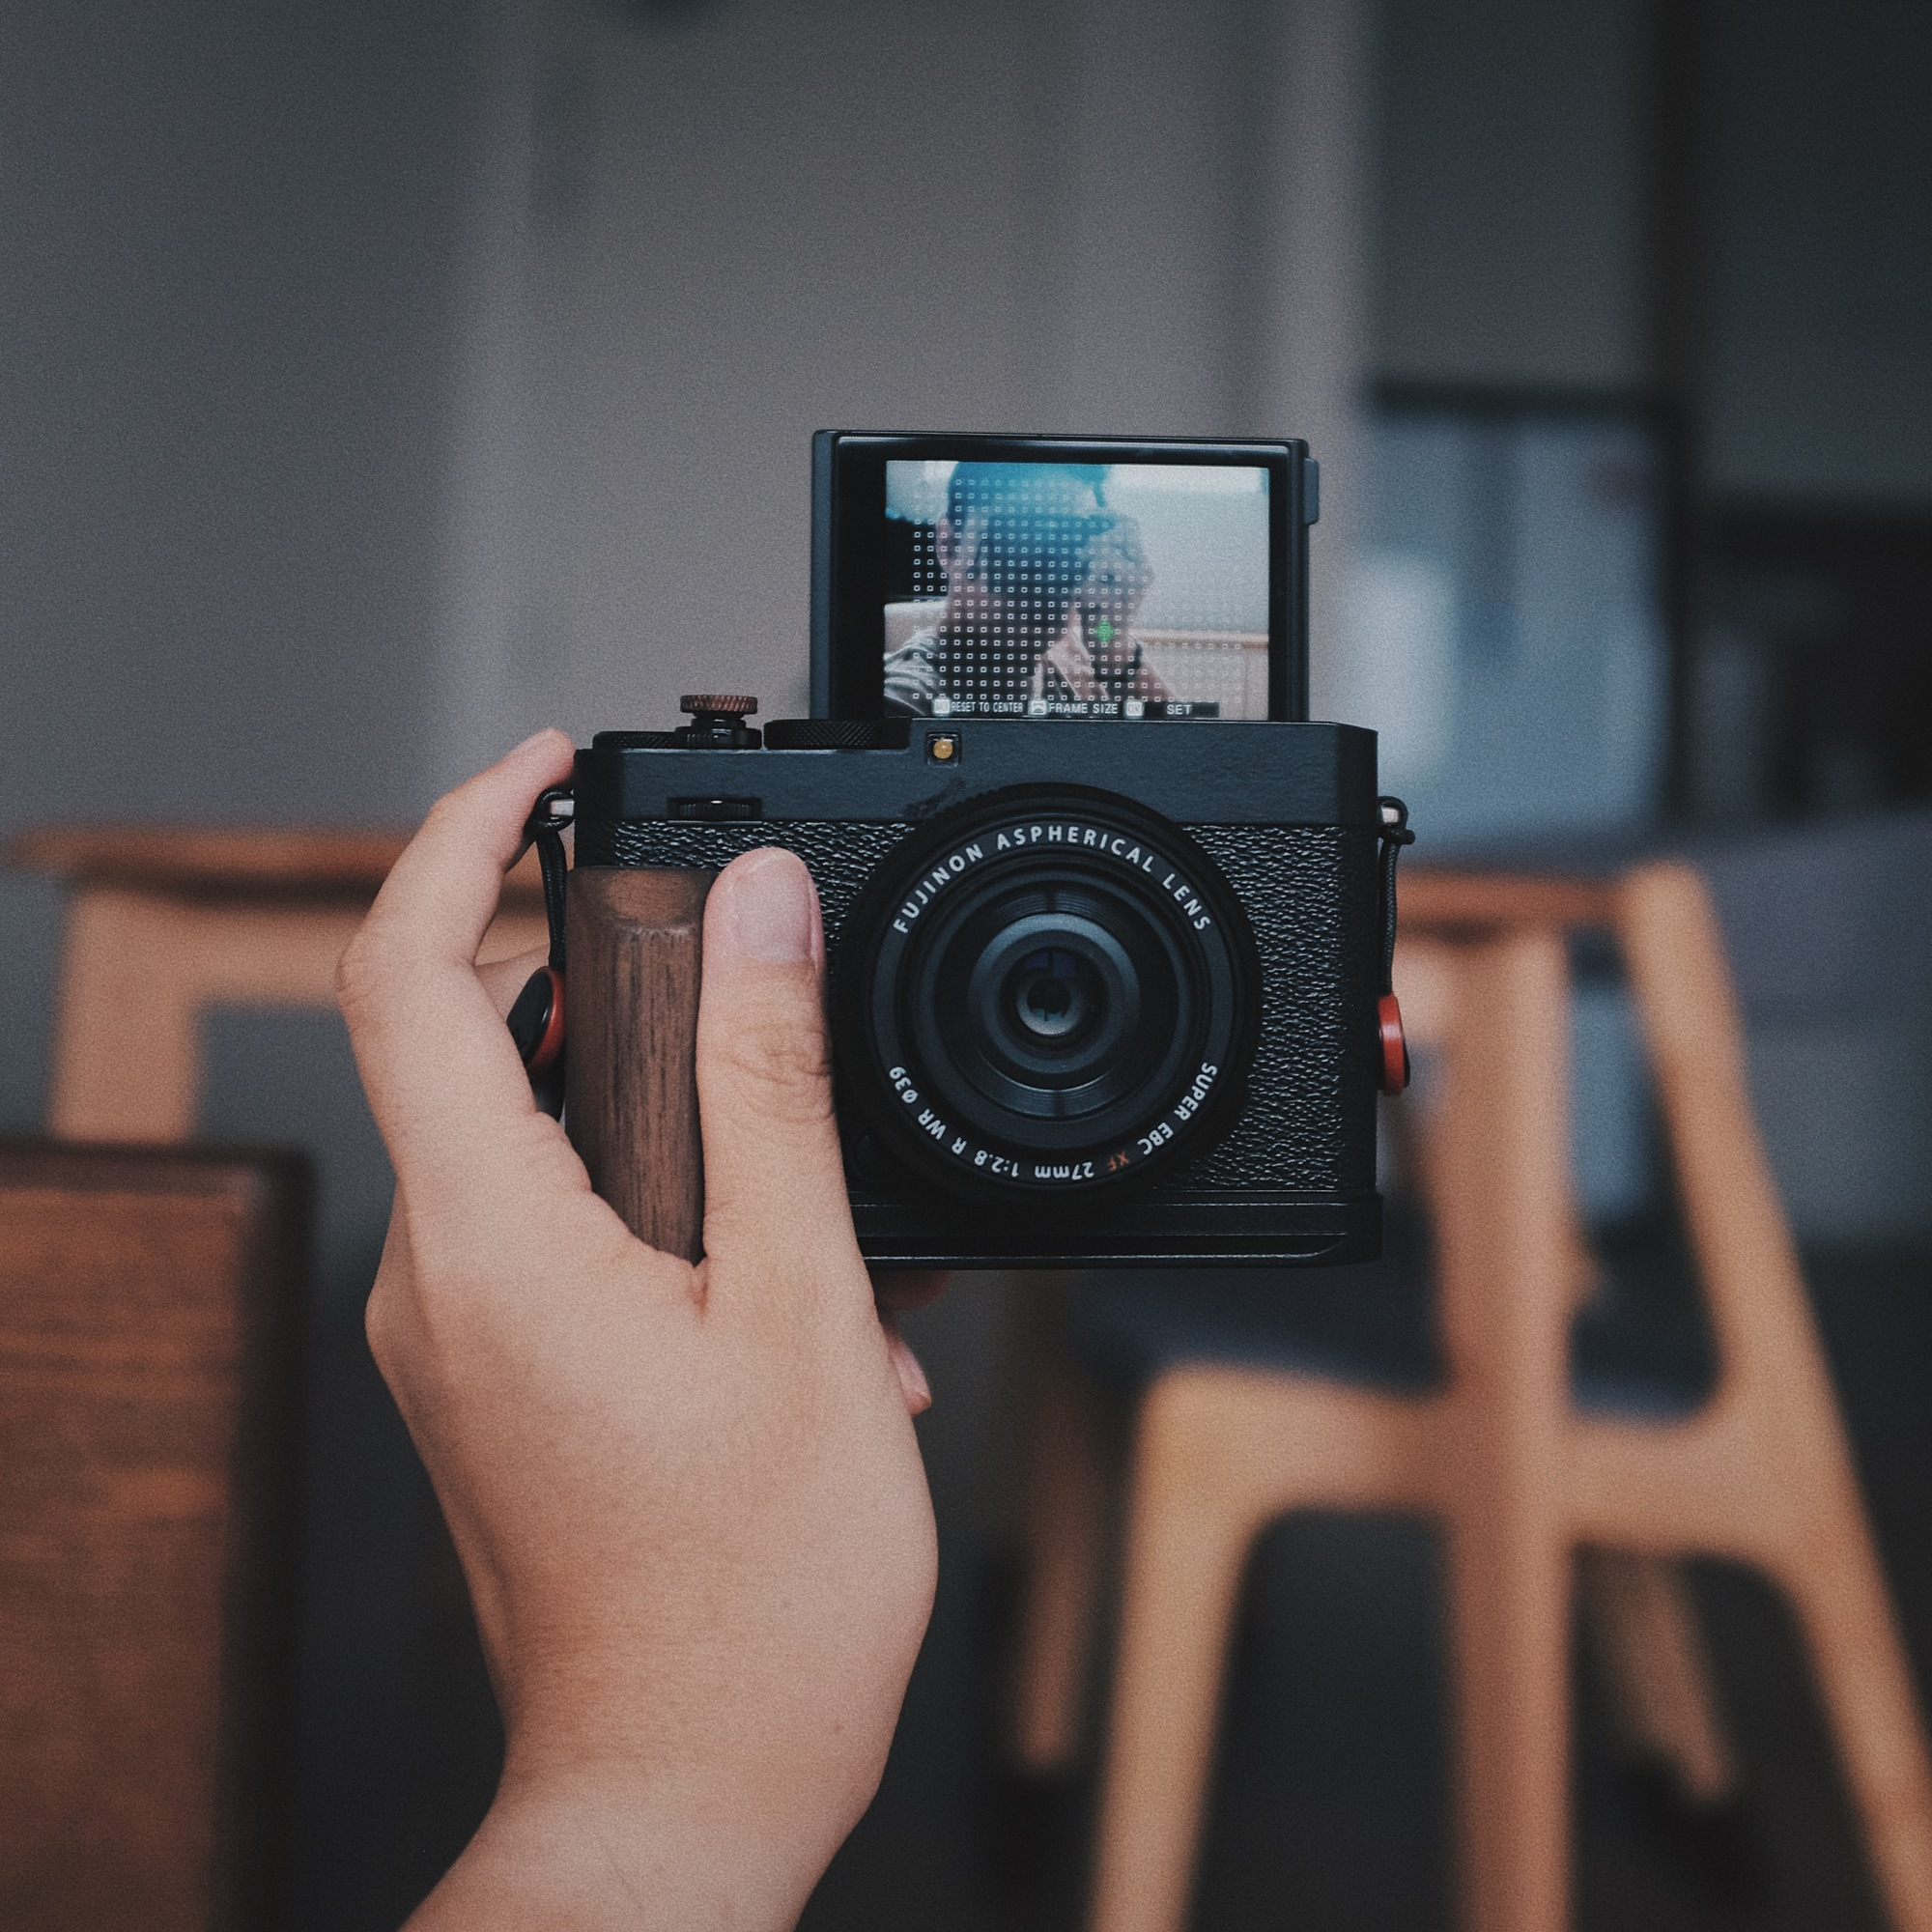
\includegraphics[width=\linewidth]{\envfinaldir/coverpic-prod.jpg}\par
            % \vskip 30pt
            \vfill

            \normalsize\rmfamily\scshape
            \copyright{} The Web Digest Project \hfill\large \envdatestr
        \end{center}
    \end{titlepage}
    % \restoregeometry
}
\newcommand{\simplehref}[1]{%
    \textcolor{blue!80!green}{\href{#1}{#1}}%
}
\renewcommand{\contentsname}{\center\Huge\sffamily\bfseries Contents\par\vskip 20pt}
\newcounter{ipartcounter}
\setcounter{ipartcounter}{0}
\newcommand{\ipart}[1]{
    % \vskip 20pt
    \clearpage
    \stepcounter{ipartcounter}
    \phantomsection
    \addcontentsline{toc}{chapter}{#1}
    % \begin{center}
    %     \Huge
    %     \sffamily\bfseries
    %     #1
    % \end{center}
    % \vskip 20pt plus 7pt
}
\newcounter{ichaptercounter}
\setcounter{ichaptercounter}{0}
\newcommand{\ichapter}[1]{
    % \vskip 20pt
    \clearpage
    \stepcounter{ichaptercounter}
    \phantomsection
    \addcontentsline{toc}{section}{\numberline{\arabic{ichaptercounter}}#1}
    \begin{center}
        \Huge
        \sffamily\bfseries
        #1
    \end{center}
    \vskip 20pt plus 7pt
}
\newcommand{\entrytitlefont}[1]{\subsection*{\raggedright\Large\sffamily\bfseries#1}}
\newcommand{\entryitemGeneric}[2]{
    % argv: title, url
    \parbox{\linewidth}{
        \entrytitlefont{#1}\par\vskip 5pt
        \footnotesize\ttfamily\mdseries
        \simplehref{#2}
    }\vskip 11pt plus 11pt minus 1pt
}
\newcommand{\entryitemGithub}[3]{
    % argv: title, url, desc
    \parbox{\linewidth}{
        \entrytitlefont{#1}\par\vskip 5pt
        \footnotesize\ttfamily\mdseries
        \simplehref{#2}\par\vskip 5pt
        \small\rmfamily\mdseries#3
    }\vskip 11pt plus 11pt minus 1pt
}
\newcommand{\entryitemAp}[3]{
    % argv: title, url, desc
    \parbox{\linewidth}{
        \entrytitlefont{#1}\par\vskip 5pt
        \footnotesize\ttfamily\mdseries
        \simplehref{#2}\par\vskip 5pt
        \small\rmfamily\mdseries#3
    }\vskip 11pt plus 11pt minus 1pt
}
\newcommand{\entryitemHackernews}[3]{
    % argv: title, hnurl, rawurl
    % \parbox{\linewidth}{
    %     \entrytitlefont{#1}\par\vskip 5pt
    %     \footnotesize\ttfamily\mdseries
    %     \simplehref{#3}\par
    %     \textcolor{black!50}{\href{#2}{#2}}
    % }\vskip 11pt plus 11pt minus 1pt
    \begin{minipage}{\linewidth}
            \entrytitlefont{#1}\par\vskip 5pt
            \footnotesize\ttfamily\mdseries
            \simplehref{#3}\par
            \textcolor{black!50}{\href{#2}{#2}}
    \end{minipage}\par\vskip 11pt plus 11pt minus 1pt
}







\begin{document}

\makeheader

\tableofcontents\clearpage




\ipart{Developers}
\ichapter{Hacker News}
\entryitemTwoLinks{Turkish university annuls Erdogan rival's degree, preventing run for president}{https://news.ycombinator.com/item?id=43404679}{https://www.reuters.com/world/asia-pacific/istanbul-university-annuls-istanbul-mayor-imamoglus-diploma-over-irregularities-2025-03-18/}

\entryitemTwoLinks{PeerTube v7.1 Is Out}{https://news.ycombinator.com/item?id=43403377}{https://joinpeertube.org/news/release-7.1}

\entryitemTwoLinks{FTC Removes Posts Critical of Amazon, Microsoft, and AI Companies}{https://news.ycombinator.com/item?id=43402957}{https://www.wired.com/story/federal-trade-commission-removed-blogs-critical-of-ai-amazon-microsoft/}

\entryitemTwoLinks{US appeals court rules AI generated art cannot be copyrighted}{https://news.ycombinator.com/item?id=43402790}{https://www.reuters.com/world/us/us-appeals-court-rejects-copyrights-ai-generated-art-lacking-human-creator-2025-03-18/}

\entryitemTwoLinks{Ask HN: How Do I Escape Homelessness After Rebuilding My Mental Health?}{https://news.ycombinator.com/item?id=43402315}{https://news.ycombinator.com/item?id=43402315}

\entryitemTwoLinks{HTTrack Website Copier}{https://news.ycombinator.com/item?id=43402149}{https://www.httrack.com/}

\entryitemTwoLinks{Amazon to kill off local Alexa processing, all voice requests shipped to cloud}{https://news.ycombinator.com/item?id=43402115}{https://www.theregister.com/2025/03/17/amazon\_kills\_on\_device\_alexa/}

\entryitemTwoLinks{Show HN: I made a tool to port tweets to Bluesky mantaining their original date}{https://news.ycombinator.com/item?id=43401855}{https://bluemigrate.com}

\entryitemTwoLinks{Fedora 42 Beta}{https://news.ycombinator.com/item?id=43401595}{https://www.redhat.com/en/blog/fedora-42-beta-now-available}

\entryitemTwoLinks{Preview: Amazon S3 Tables and Lakehouse in DuckDB}{https://news.ycombinator.com/item?id=43401421}{https://duckdb.org/2025/03/14/preview-amazon-s3-tables.html}

\entryitemTwoLinks{Apple restricts Pebble from being awesome with iPhones}{https://news.ycombinator.com/item?id=43401245}{https://ericmigi.com/blog/apple-restricts-pebble-from-being-awesome-with-iphones/}

\entryitemTwoLinks{Designing Electronics That Work}{https://news.ycombinator.com/item?id=43401179}{https://www.hscott.net/designing-electronics-that-work/}

\entryitemTwoLinks{Two new PebbleOS watches}{https://news.ycombinator.com/item?id=43400989}{https://ericmigi.com/blog/introducing-two-new-pebbleos-watches/}

\entryitemTwoLinks{The real failure rate of EBS}{https://news.ycombinator.com/item?id=43399811}{https://planetscale.com/blog/the-real-fail-rate-of-ebs}

\entryitemTwoLinks{North Korea Launders Billions in Stolen Crypto}{https://news.ycombinator.com/item?id=43399190}{https://www.coindesk.com/policy/2025/03/07/here-s-how-north-korea-launders-billions-of-stolen-crypto}

\entryitemTwoLinks{Half-Life 2 RTX}{https://news.ycombinator.com/item?id=43399168}{https://store.steampowered.com/app/2477290/HalfLife\_2\_RTX/}

\entryitemTwoLinks{Wired is dropping paywalls for FOIA-based reporting. Others should follow}{https://news.ycombinator.com/item?id=43399138}{https://freedom.press/issues/wired-is-dropping-paywalls-for-foia-based-reporting-others-should-follow/}

\entryitemTwoLinks{Java 24}{https://news.ycombinator.com/item?id=43398999}{https://jdk.java.net/24/}

\entryitemTwoLinks{Google announces agreement to acquire Wiz}{https://news.ycombinator.com/item?id=43398780}{https://blog.google/inside-google/company-announcements/google-agreement-acquire-wiz/}

\entryitemTwoLinks{Stamina Is a Quiet Advantage}{https://news.ycombinator.com/item?id=43398589}{https://kupajo.com/stamina-is-a-quiet-advantage/}\ichapter{Phoronix}
\entryitemGeneric{\hskip 0pt{}NVIDIA 570.133.07 Linux Driver Released With A Few Fixes}{https://www.phoronix.com/news/NVIDIA-570.133.07-Linux-Driver}

\entryitemGeneric{\hskip 0pt{}Asahi Lina Pausing Work On Apple GPU Linux Driver Development}{https://www.phoronix.com/news/Asahi-Lina-Steps-Down-Linux-GPU}

\entryitemGeneric{\hskip 0pt{}Ubuntu Developers Discuss Abandoning Mailing Lists For Discourse}{https://www.phoronix.com/news/Ubuntu-Mailing-Lists-Discourse}

\entryitemGeneric{\hskip 0pt{}BLAKE3 1.7 Turns To Intel's oneTBB For Parallelizing C Code - Similar Perf To Rust+Rayon}{https://www.phoronix.com/news/BLAKE3-1.7-Released}

\entryitemGeneric{\hskip 0pt{}Final Draft Of PCI Express 7.0 Specification Published}{https://www.phoronix.com/news/PCI-Express-7.0-v0.9}

\entryitemGeneric{\hskip 0pt{}Blender 4.4 Released With Vulkan Improvements \& AMD HIP RT No Longer Experimental}{https://www.phoronix.com/news/Blender-4.4-Released}

\entryitemGeneric{\hskip 0pt{}OpenJDK Java 24 Released With Garbage Collector Improvements, Deprecating x86 32-bit}{https://www.phoronix.com/news/OpenJDK-Java-24-Released}

\entryitemGeneric{\hskip 0pt{}Fedora 42 Beta Released With Countless Improvements}{https://www.phoronix.com/news/Fedora-42-Beta}

\entryitemGeneric{\hskip 0pt{}Linux Kernel's Zstd Code Gets A Co-Maintainer}{https://www.phoronix.com/news/Linux-Zstd-Co-Maintainer}\ichapter{Dribbble}
\entryitemGeneric{\hskip 0pt{}Crypto Bridge}{https://dribbble.com/shots/25783744-Crypto-Bridge}

\entryitemGeneric{\hskip 0pt{}Rose Logo Design [for sale]}{https://dribbble.com/shots/25775027-Rose-Logo-Design-for-sale}

\entryitemGeneric{\hskip 0pt{}Mammut Logo Redesign Concept}{https://dribbble.com/shots/25776663-Mammut-Logo-Redesign-Concept}

\entryitemGeneric{\hskip 0pt{}DL}{https://dribbble.com/shots/25775198-DL}

\entryitemGeneric{\hskip 0pt{}Cimet Logo Grid}{https://dribbble.com/shots/25710567-Cimet-Logo-Grid}

\entryitemGeneric{\hskip 0pt{}Abstract S Logo Design // For Sale}{https://dribbble.com/shots/25764643-Abstract-S-Logo-Design-For-Sale}

\entryitemGeneric{\hskip 0pt{}Protec Recovery Logo Design}{https://dribbble.com/shots/25764203-Protec-Recovery-Logo-Design}

\entryitemGeneric{\hskip 0pt{}Spin}{https://dribbble.com/shots/25765149-Spin}

\entryitemGeneric{\hskip 0pt{}Fintech icons pack part 3 for download}{https://dribbble.com/shots/25728645-Fintech-icons-pack-part-3-for-download}

\entryitemGeneric{\hskip 0pt{}Capobara}{https://dribbble.com/shots/25764582-Capobara}

\entryitemGeneric{\hskip 0pt{}Triceratops}{https://dribbble.com/shots/25761010-Triceratops}

\entryitemGeneric{\hskip 0pt{}Tab Bar Animation}{https://dribbble.com/shots/25760227-Tab-Bar-Animation}

\entryitemGeneric{\hskip 0pt{}Chief Logo Design Process}{https://dribbble.com/shots/25759736-Chief-Logo-Design-Process}

\entryitemGeneric{\hskip 0pt{}World Clock App Design}{https://dribbble.com/shots/25760174-World-Clock-App-Design}

\entryitemGeneric{\hskip 0pt{}Flare - Logo Design 2}{https://dribbble.com/shots/25760645-Flare-Logo-Design-2}

\entryitemGeneric{\hskip 0pt{}Columbus Lions®}{https://dribbble.com/shots/25761563-Columbus-Lions}

\entryitemGeneric{\hskip 0pt{}Carbon Solutions B2B Dashboard Design}{https://dribbble.com/shots/25681782-Carbon-Solutions-B2B-Dashboard-Design}

\entryitemGeneric{\hskip 0pt{}Flare - Logo Design 🚀}{https://dribbble.com/shots/25754585-Flare-Logo-Design}

\entryitemGeneric{\hskip 0pt{}Bir-D / D.Bird}{https://dribbble.com/shots/25757221-Bir-D-D-Bird}

\entryitemGeneric{\hskip 0pt{}Logowave Awards Entry from Lepisov Branding}{https://dribbble.com/shots/25755190-Logowave-Awards-Entry-from-Lepisov-Branding}

\entryitemGeneric{\hskip 0pt{}Squid Book}{https://dribbble.com/shots/25756273-Squid-Book}

\entryitemGeneric{\hskip 0pt{}Order detail dashboard}{https://dribbble.com/shots/25748173-Order-detail-dashboard}

\entryitemGeneric{\hskip 0pt{}Pricing Plan Web Page Design}{https://dribbble.com/shots/25755045-Pricing-Plan-Web-Page-Design}

\entryitemGeneric{\hskip 0pt{}Bounce}{https://dribbble.com/shots/25755477-Bounce}


\ipart{Developers~~~~(zh-Hans)}
\ichapter{Solidot}
\entryitemGeneric{\hskip 0pt{}欧洲科技公司呼吁欧盟推动购买欧洲科技产品}{https://www.solidot.org/story?sid=80821}

\entryitemGeneric{\hskip 0pt{}人类的脑力已经越过峰值?}{https://www.solidot.org/story?sid=80820}

\entryitemGeneric{\hskip 0pt{}周五是否应该成为新的周六?}{https://www.solidot.org/story?sid=80819}

\entryitemGeneric{\hskip 0pt{}哈佛对年收入 20 万美元以内家庭免除学费}{https://www.solidot.org/story?sid=80818}

\entryitemGeneric{\hskip 0pt{}百度副总裁的未成年女儿被指参与开盒}{https://www.solidot.org/story?sid=80817}

\entryitemGeneric{\hskip 0pt{}Google 在 AI 训练数据集的版权问题上与 OpenAI 意见一致}{https://www.solidot.org/story?sid=80816}

\entryitemGeneric{\hskip 0pt{}特斯拉二手车价格下跌}{https://www.solidot.org/story?sid=80815}

\entryitemGeneric{\hskip 0pt{}华为计划在 Windows 授权过期后转向 Linux}{https://www.solidot.org/story?sid=80814}

\entryitemGeneric{\hskip 0pt{}网信办等发布《人工智能生成合成内容标识办法》}{https://www.solidot.org/story?sid=80813}

\entryitemGeneric{\hskip 0pt{}GIMP 3.0 释出}{https://www.solidot.org/story?sid=80812}

\entryitemGeneric{\hskip 0pt{}Gemini 将在今年晚些时候取代 Google Assistant}{https://www.solidot.org/story?sid=80811}

\entryitemGeneric{\hskip 0pt{}tj-actions 供应链攻击暴露大企业秘密}{https://www.solidot.org/story?sid=80810}

\entryitemGeneric{\hskip 0pt{}波音宇航员将于 3 月 18 日返回地面}{https://www.solidot.org/story?sid=80809}

\entryitemGeneric{\hskip 0pt{}我们的宇宙是否困在一个黑洞中?}{https://www.solidot.org/story?sid=80808}

\entryitemGeneric{\hskip 0pt{}屏幕时间与心血管病风险上升相关}{https://www.solidot.org/story?sid=80807}

\entryitemGeneric{\hskip 0pt{}Blue Ghost 探测器记录到日全食}{https://www.solidot.org/story?sid=80806}

\entryitemGeneric{\hskip 0pt{}七大科技公司推动中国股市上涨}{https://www.solidot.org/story?sid=80805}

\entryitemGeneric{\hskip 0pt{}中国五岁以下儿童可避免死亡率过去几十年显著下降}{https://www.solidot.org/story?sid=80804}

\entryitemGeneric{\hskip 0pt{}水中有氧运动有助于减肥}{https://www.solidot.org/story?sid=80803}

\entryitemGeneric{\hskip 0pt{}Waymo 的无人出租车去年在旧金山收到了 589 张违反停车规定的罚单}{https://www.solidot.org/story?sid=80802}\ichapter{V2EX}
\entryitemGeneric{\hskip 0pt{}[电动汽车] byd 1000kw 怎么做到的}{https://www.v2ex.com/t/1119486}

\entryitemGeneric{\hskip 0pt{}[OpenAI] 最近高强度使用 ChatGPT 和 Claude 时发现的一些变化}{https://www.v2ex.com/t/1119481}

\entryitemGeneric{\hskip 0pt{}[macOS] 复制 mac 中文件到 webdav 等网络磁盘中会出现 .\_xxx 的文件}{https://www.v2ex.com/t/1119480}

\entryitemGeneric{\hskip 0pt{}[YouTube] 国内如何观看 YouTube Kids(不折腾版)}{https://www.v2ex.com/t/1119479}

\entryitemGeneric{\hskip 0pt{}[Android] QQ 邮箱 Android 客户端推送问题}{https://www.v2ex.com/t/1119478}

\entryitemGeneric{\hskip 0pt{}[分享创造] 我做了一个 manus 的指南网站}{https://www.v2ex.com/t/1119477}

\entryitemGeneric{\hskip 0pt{}[程序员] 请教消息队列的选择}{https://www.v2ex.com/t/1119476}

\entryitemGeneric{\hskip 0pt{}[Apple] 有没有免费的锁屏启动软件}{https://www.v2ex.com/t/1119475}

\entryitemGeneric{\hskip 0pt{}[大学] 中下 985 软件工程专业,对升学/就业纠结万分,内心很痛苦}{https://www.v2ex.com/t/1119474}

\entryitemGeneric{\hskip 0pt{}[问与答] 求 manus 注册教程}{https://www.v2ex.com/t/1119471}

\entryitemGeneric{\hskip 0pt{}[随想] 我理解的 MCP 是一个 AI 和万物互联的协议标准,未来已来。}{https://www.v2ex.com/t/1119470}

\entryitemGeneric{\hskip 0pt{}[VPS] 甲骨文云 ip ping 不通, ssh 能连上,是被墙了吗}{https://www.v2ex.com/t/1119469}

\entryitemGeneric{\hskip 0pt{}[Android] 能否用小爱同学 点播我手机本地的歌?}{https://www.v2ex.com/t/1119468}

\entryitemGeneric{\hskip 0pt{}[随想] 不久的将来会不会有 ai 监工}{https://www.v2ex.com/t/1119467}

\entryitemGeneric{\hskip 0pt{}[Android] 在系统语言为英文时,什么开屏广告跳过工具效果最好?}{https://www.v2ex.com/t/1119465}

\entryitemGeneric{\hskip 0pt{}[分享发现] 我办了中国移动的云电脑, 太狗血了, 说出来给大家乐一下,}{https://www.v2ex.com/t/1119463}

\entryitemGeneric{\hskip 0pt{}[Apple] 两台 Mac 如何共享显示器?}{https://www.v2ex.com/t/1119460}

\entryitemGeneric{\hskip 0pt{}[酷工作] [广州][已盈利出海应用]招聘前端开发工程师\&产品经理管培生}{https://www.v2ex.com/t/1119459}

\entryitemGeneric{\hskip 0pt{}[macOS] brew install 为什么 intel 芯片和 m 芯片差别这么大}{https://www.v2ex.com/t/1119458}

\entryitemGeneric{\hskip 0pt{}[iPhone] 12pm 电池健康 71,如何换原装电池性价比最高}{https://www.v2ex.com/t/1119457}

\entryitemGeneric{\hskip 0pt{}[问与答] 小店收银系统求推荐}{https://www.v2ex.com/t/1119456}

\entryitemGeneric{\hskip 0pt{}[生活] 《人生首次交通事故,经过有点恶心》受害者视角}{https://www.v2ex.com/t/1119455}

\entryitemGeneric{\hskip 0pt{}[分享创造] V2EX 处女贴:我绘制了最近 20 年的中国工作日日历,看看这些年节假日都有什么变化}{https://www.v2ex.com/t/1119454}

\entryitemGeneric{\hskip 0pt{}[问与答] 三方店买的 tplink 有什么猫腻吗?}{https://www.v2ex.com/t/1119452}

\entryitemGeneric{\hskip 0pt{}[职场话题] 硬件工程师待遇为何不如软件工程师?}{https://www.v2ex.com/t/1119451}

\entryitemGeneric{\hskip 0pt{}[分享创造] 分享我们的新博客主题,以及欢迎大家分享自己的博客}{https://www.v2ex.com/t/1119450}

\entryitemGeneric{\hskip 0pt{}[NAS] 硬盘空间真不耐存,一部绝命毒师就 0.5 个 t 了,刚榨干核显装的 jellyfin 索然无味,求个 nas 机箱}{https://www.v2ex.com/t/1119449}

\entryitemGeneric{\hskip 0pt{}[Apple] 各位有遇到过输入法自己变了的情况吗?}{https://www.v2ex.com/t/1119448}

\entryitemGeneric{\hskip 0pt{}[生活] 借 V 站替姐姐相亲一下,走过路过别错过。-----后续}{https://www.v2ex.com/t/1119447}

\entryitemGeneric{\hskip 0pt{}[问与答] 求助,关于 CloudFlare 和 DDNS 的问题}{https://www.v2ex.com/t/1119446}

\entryitemGeneric{\hskip 0pt{}[Rust] 求帮打包个 exe}{https://www.v2ex.com/t/1119445}

\entryitemGeneric{\hskip 0pt{}[问与答] 如果有这么一个 信息流管理工具,你们会用吗}{https://www.v2ex.com/t/1119444}

\entryitemGeneric{\hskip 0pt{}[淘宝] 淘宝看不到详情页是什么情况?}{https://www.v2ex.com/t/1119443}

\entryitemGeneric{\hskip 0pt{}[Apple] 请问大佬, m4 MacBook Air 外接 2k 显示器刷新率只能 60hz 吗??}{https://www.v2ex.com/t/1119442}

\entryitemGeneric{\hskip 0pt{}[macOS] 新发现🌟 如果你有两台 mac 的话,可以将其中一台 mac 作为拓展显示器}{https://www.v2ex.com/t/1119441}

\entryitemGeneric{\hskip 0pt{}[分享创造] 我做了一个 AI SaaS 图像处理平台 https://removeshadow.com}{https://www.v2ex.com/t/1119440}

\entryitemGeneric{\hskip 0pt{}[macOS] 请教一下各位 mac 用户。请问如何批量修改相同后缀的文件的图标?}{https://www.v2ex.com/t/1119439}

\entryitemGeneric{\hskip 0pt{}[TypeScript] typescript 达人乱入}{https://www.v2ex.com/t/1119438}

\entryitemGeneric{\hskip 0pt{}[分享创造] 一个 AI 产品 Affiliate Program 导航站}{https://www.v2ex.com/t/1119437}

\entryitemGeneric{\hskip 0pt{}[程序员] Python 的 faker 库是不是有问题}{https://www.v2ex.com/t/1119435}

\entryitemGeneric{\hskip 0pt{}[macOS] 现在的 OneDrive 会把始终保留在本地的文件存两遍}{https://www.v2ex.com/t/1119434}

\entryitemGeneric{\hskip 0pt{}[Android] 如何屏蔽 app 检测系统语言设置}{https://www.v2ex.com/t/1119433}

\entryitemGeneric{\hskip 0pt{}[VPS] ucloud 国内服务器,联通线路被封禁}{https://www.v2ex.com/t/1119432}

\entryitemGeneric{\hskip 0pt{}[问与答] 如何删除过去用微博图床上传到微博的图片?找不到删除接口。}{https://www.v2ex.com/t/1119431}

\entryitemGeneric{\hskip 0pt{}[iPhone] 香港地铁🚇3/22 开始支持『交通联合』卡,那么问题来了,假设 iPhone 上同时有『深圳通交联版』和『八达通』,还能自动切换吗?🌚}{https://www.v2ex.com/t/1119428}

\entryitemGeneric{\hskip 0pt{}[iOS] FaceTime 中无法识别联系人为蓝色,但是 iMessage 中相同联系人可以正常识别为蓝色。}{https://www.v2ex.com/t/1119426}

\entryitemGeneric{\hskip 0pt{}[分享创造] 我也分享一个匿名匹配聊天的工具}{https://www.v2ex.com/t/1119425}

\entryitemGeneric{\hskip 0pt{}[V2EX] v 站可以支持一下黑夜模式吗}{https://www.v2ex.com/t/1119422}

\entryitemGeneric{\hskip 0pt{}[OpenWrt] openwrt 去广告的方案}{https://www.v2ex.com/t/1119421}

\entryitemGeneric{\hskip 0pt{}[Windows] Windows 又在犯大病了}{https://www.v2ex.com/t/1119420}


\ipart{Generic News}







\clearpage
\leavevmode\vfill
\footnotesize

Copyright \copyright{} 2023-2025 Neruthes and other contributors.

This document is published with CC BY-NC-ND 4.0 license.

The entries listed in this newsletter may be copyrighted by their respective creators.

This newsletter is generated by the Web Digest project.

The newsletters are also delivered via Telegram channel \CJKunderline{\href{https://t.me/webdigestchannel}{https://t.me/webdigestchannel}}.\\
RSS feed is available at \CJKunderline{\href{https://webdigest.pages.dev/rss.xml}{https://webdigest.pages.dev/rss.xml}}.

This newsletter is available in PDF at
\CJKunderline{\href{https://webdigest.pages.dev/}{https://webdigest.pages.dev/}}.

The source code being used to generate this newsletter is available at\\
\CJKunderline{\href{https://github.com/neruthes/webdigest}{https://github.com/neruthes/webdigest}}.

This newsletter is also available in
\CJKunderline{\href{http://webdigest.pages.dev/readhtml/\envyear/WebDigest-20250319.html}{HTML}} and
\CJKunderline{\href{https://github.com/neruthes/webdigest/blob/master/markdown/\envyear/WebDigest-20250319.md}{Markdown}}.


\coverpic{https://unsplash.com/photos/city-buildings-at-night-with-lights-on-kiBol35Fmx8}{Josh Hild}


\end{document}
